
\FloatBarrier
\section{Система с сухим трением} %  % {{{1  __FRIC__
\label{atu:sect:fric}

\LinkRef{
  fric: ASAU-11, DSMP-2016
}

\subsection{Определение системы и анализ её динамики} %  % {{{2 _fric_task


Существуют динамические системы, не обладающие хаотическим поведением,
которые, тем не менее, проявляют сходные свойства с точки зрения идентификации.
А именно, непосредственное сравнение выходов системы и модели не позволяет
сделать никаких выводов о соотношениях между параметрами модели и объекта.
Одним из примеров таких систем является динамическая система (\ref{atu:eq:dryfric_sys}),
моделирующая поведение тела заданной массы по действием внешней вынуждающей силы
и силы сухого трения
\cite{berger_friction,osn_dyn_prom_robot,borcov}:
%
\begin{equation}
  m \ddot{x} + f_{df}( x, \dot{x}, \ldots)  = u(t).
\label{atu:eq:dryfric_sys}
\end{equation}
%
%\noindent
где
$m$ -- масса тела,
$u(t)$ -- вынуждающая сила,
$ f_{df}( x, \dot{x}, \ldots)  $ -- сила сухого трения.

Важной особенностью при моделировании силы сухого трения является тот факт,
что это силу невозможно корректно выразить аналитически~\cite{atu_asau11}. Более того,
её алгоритмическое представления неизбежно потребует учёта всех других сил,
действующих на тело, то крайней мере, для корректного представления
силы трения покоя. Эта особенность не даёт возможности
аналитического анализа таких систем, за исключением ограниченного набора
вырожденных случаев. При этом, такое поведение существенно затрудняет идентификацию,
и, в определённых случая, делает её принципиально невозможной.

Основным параметром, в простейшем случае определяющим силу сухого
трения, является $f_{dm}$ -- максимальная значение её модуля.
Определение этой величины и будем считать целью задачи идентификации
системы с сухим трением.

В свою очередь, существенным свойством данной системы является то, что в каждой точке \(x\)
система может находится в покое, даже если на неё действует
внешняя сила (по модулю не превышающая $f_{dm}$).
Если же рассмотреть пару или более подобных систем,
то получившаяся система имеет общие свойства с системами
хаотической динамики, а именно: малые возмущения входного сигнала
или коэффициентов модели приводят к значительным изменениям
выходного, причем реакция на возмущения может быть
не ограничена во времени.
Более того, даже если после какого-то момента времени
параметры объекта и коэффициенты модели полностью совпадут,
величина ошибки по выходнам не устремится к нулю, а останется на прежнем уровне.

На рис.~\ref{atu:f:fric_outs} представлен сравнительный пример динамики трёх
моделей, при одинаковом входном сигнале
и различных значениях $f_{dm}$.

\begin{figure}[htb!]
  \centerline{
    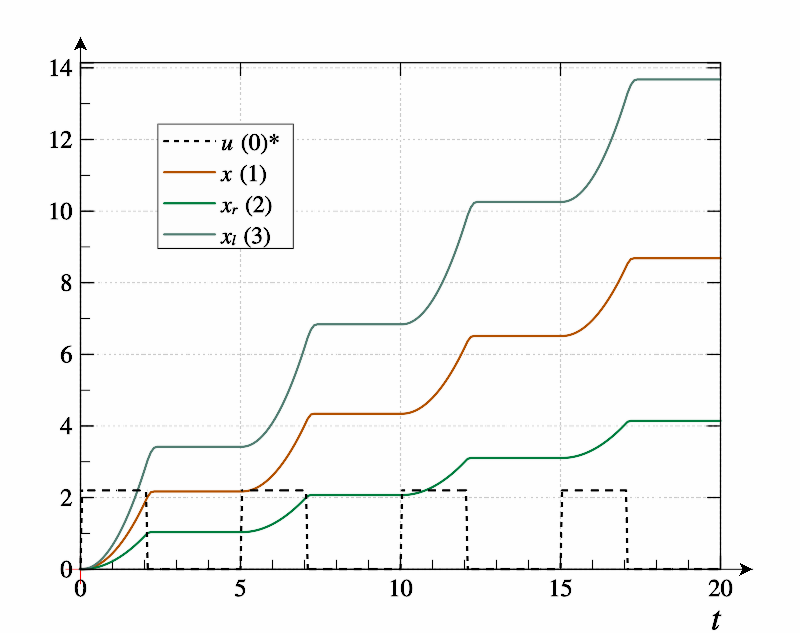
\includegraphics[width=0.5\textwidth]{p/cha/fric/fric_outs1.png}
  }
  \caption{Динамика трёх моделей вида (\ref{atu:eq:dryfric_sys})}
  \label{atu:f:fric_outs}
\end{figure}

При дальнейшем моделировании, в качестве сигнала $u(t)$ использовался кусочно-линейный периодический сигнал,
в котором чередуются ``плато'' и резкие изменения. Выбор такой формы обусловлен
характерными режимами работы систем позиционирования электромеханических
устройств, для которых и характерно влияние сухого трения.

% }}}2

\subsection{Анализ и выбор критериев}  % {{{2

Для обеспечения возможности применения методов идентификации,
необходимо существование критерия
\( q(x(t)) \),
удовлетворяющего следующим требованиям:

\begin{itemize}

\item
чувствительность к \textit{динамике} модели и объекта;

\item
свойство астатизма, то есть
независимость
от смещения выхода объекта или модели:
\( q(x(t)+a ) \approx q( x(t) ) \);

\item
достаточная устойчивость к шумам измерения;

\item
физическая реализуемость.

\end{itemize}

Первые два требования
могут быть достигнуты путём вычисления производной --
скорости изменения выходных сигналов
\(v = \mathrm{d}\,x(t)/ \mathrm{d}\,t \),
и формирования критерия идентификации на её основе.

Однако, при этом система становится исключительно чувствительной
к шумам измерения. Даже в том случае, когда
оценка производной производится физически реализуемыми методами,
создать работоспособную систему идентификации на основе критериев
подобного вида практически невозможно.

В работе \cite{atu_asau11} был предложен метод синтеза критерия идентификации
на основе гистерезисной фильтрации выходных сигналов, с последующим
вычислением производной. Метод показал свою работоспособность, однако,
он требует достаточно точных сведений об уровне и виде шумов -- для
настройки гистерезисного фильтра. В данной работе сделаем предположение,
что уровень шумов позволяет создать фильтр, позволяющий отсеивать шумы
за (как максимум) характерное время реакции системы.
После фильтра действует реальное дифференцирующее звено.
Соответствующий вид критерия обозначим как $ q_\mathrm{dx} $ (рис.~\ref{atu:f:fric_q}).



\begin{figure}[htb!]
\centerline{
  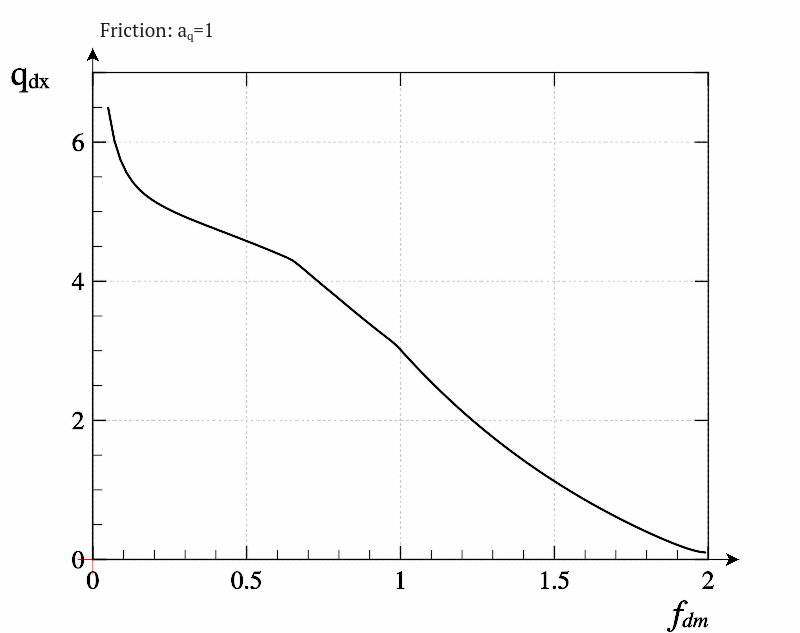
\includegraphics[width=0.60\textwidth]{p/cha/fric/fric_q-p_f_dm_q.png}
}
  \caption{Зависимость $q_\mathrm{dx}(f_{dm})$ для системы (\ref{atu:eq:dryfric_sys}) }
\label{atu:f:fric_q}
\end{figure}

Несмотря на выраженную нелинейность в начальной части графика,
данный критерий представляется вполне применимым для задачи идентификации,
ввиду монотонности ограниченным диапазоном производной.
При больших значениях параметра $f_{dm}$ смысл этого критерия теряется,
так как отсутствует динамика системы. При малых значениях возможности идентификации
тоже сильно ограничены, так как динамика системы больше определяется
массой объекта, чем пренебрежимо малой силой трения.

% }}}2


\subsection{Тестовая задача идентификации }   % {{{2

Аналогично уже рассмотренным система
определим тестовую задачу следующим образом:
\[
  f_{dm}(t) \equiv p_o(t) \in (0.1, 1.5),
\]
%
\begin{equation}
  p_o(t) = p_0 +  U_{p} \sign \sin( \omega_{p} t ),
  \label{atu:eq:fric_po_t_sign}
\end{equation}
%
%
\begin{equation}
  p_o(t) = p_0 +  U_{p} \sin( \omega_{p} t ),
  \label{atu:eq:fric_po_t_sin}
\end{equation}
%
где:
$p_0 = 0.7$, $U_p=0.4$, $\omega_p=0.0104719755$.

Динамика процессов идентификации для системы (\ref{atu:eq:dryfric_sys})
с использованием группы методов ql3rlWvnAAW.$q_\mathrm{dx}$
при условии (\ref{atu:eq:fric_po_t_sign})
представлена на рис.~\ref{atu:f:fric_id_ql3rlWvnAAW_q_dx_sign}.


\begin{figure}[htb!]
  \centerline{
    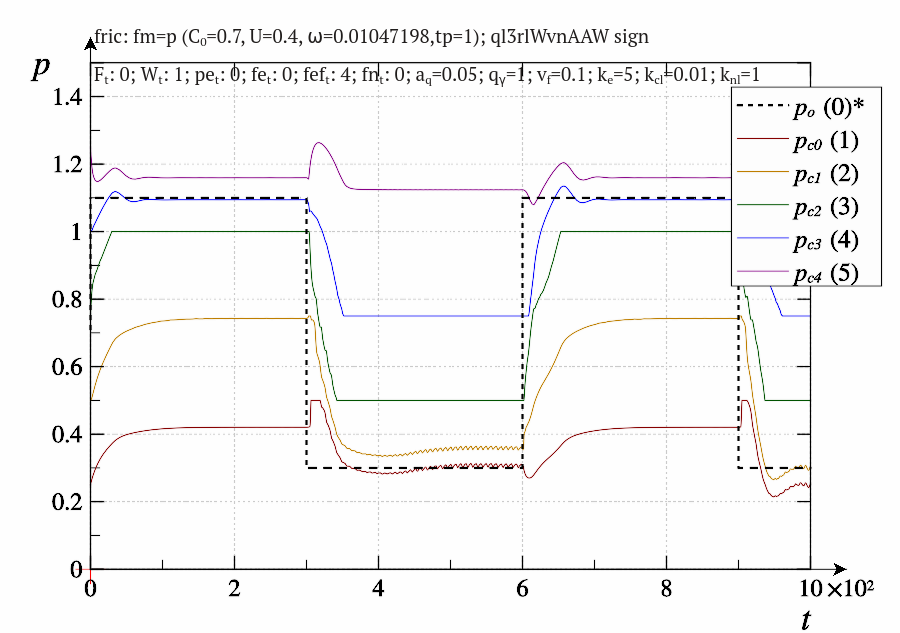
\includegraphics[width=0.49\textwidth]{p/cha/fric/ql3rlWvnAAW/fric_id-p_t_pi_ql3rlWvnAAW_sign.png}
    \hfill
    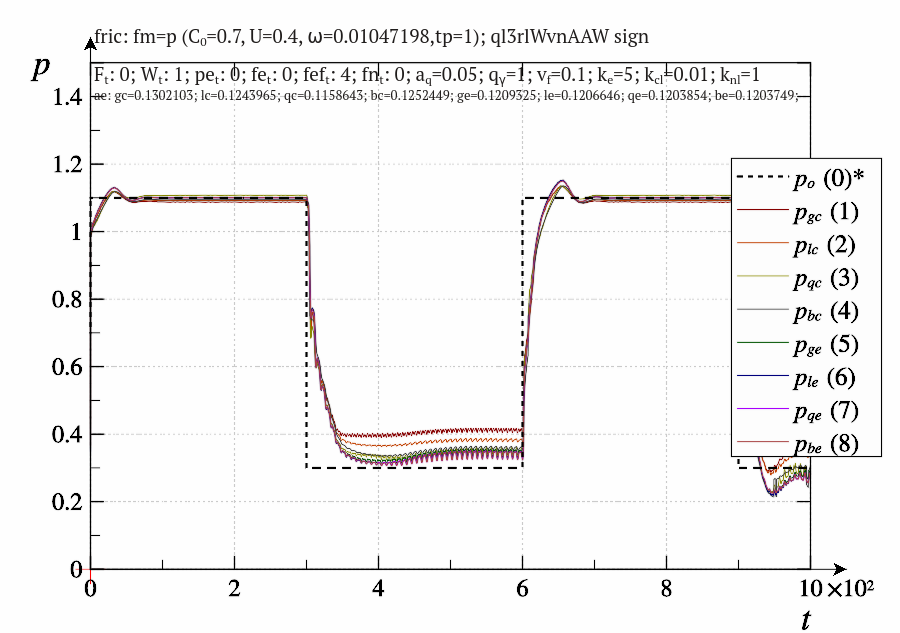
\includegraphics[width=0.49\textwidth]{p/cha/fric/ql3rlWvnAAW/fric_id-p_t_p_ql3rlWvnAAW_sign.png}
  }
  \caption{Процесс идентификации параметра ``$f_{dm}$'' системы (\ref{atu:eq:dryfric_sys}) группой методов ql3rlWvnAAW.$q_\mathrm{dx}$ при условии~(\ref{atu:eq:fric_po_t_sign})}
  \label{atu:f:fric_id_ql3rlWvnAAW_q_dx_sign}
\end{figure}

Для рассматриваемых условий наблюдается малый уровень возмущений
идентифицируемого параметра. Однако, при малых значениях $f_{dm}$
наблюдается заметная статическая ошибка идентификации. Это связано с тем,
что в этой области влияние трения становится мало,
и критерий теряет свою адекватность.

Следует отметить, что при
больших значениях $\omega_p$ наблюдается
сильное влияние входного сигнала, В силу того, что когда системы неподвижны
на одном из ``плато'', в эти моменты нет возможности различить их параметры,
какой бы критерий при этом не использовался.

Результаты моделирования при аналогичных условиях, но
при динамике параметра, заданной (\ref{atu:eq:fric_po_t_sin}),
представлены на рис.~\ref{atu:f:fric_id_ql3rlWvnAAW_q_dx_sin}.

\begin{figure}[htb!]
  \centerline{
    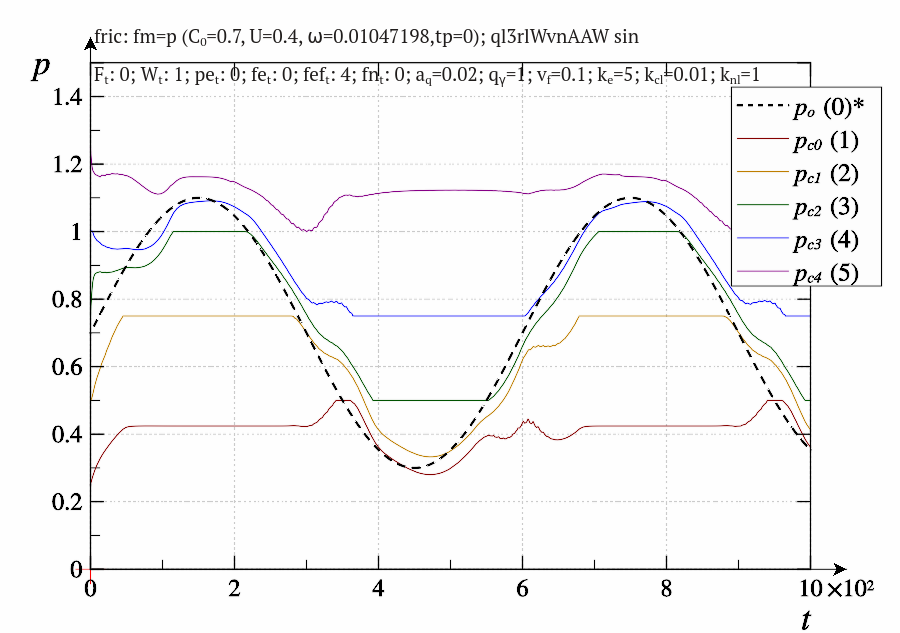
\includegraphics[width=0.49\textwidth]{p/cha/fric/ql3rlWvnAAW/fric_id-p_t_pi_ql3rlWvnAAW_sin.png}
    \hfill
    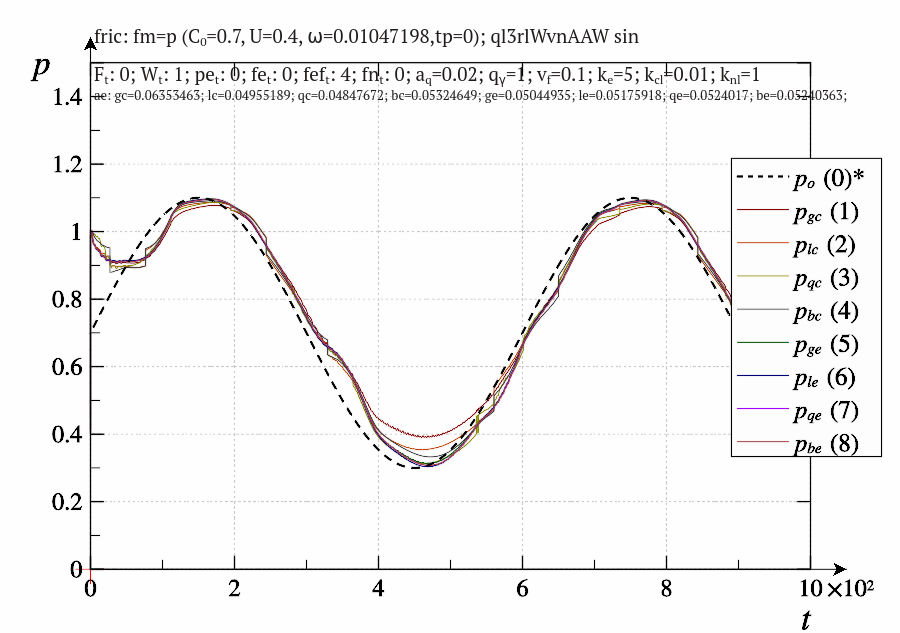
\includegraphics[width=0.49\textwidth]{p/cha/fric/ql3rlWvnAAW/fric_id-p_t_p_ql3rlWvnAAW_sin.png}
  }
  \caption{Процесс идентификации параметра ``$f_{dm}$'' системы (\ref{atu:eq:dryfric_sys}) группой методов ql3rlWvnAAW.$q_\mathrm{dx}$ при условии~(\ref{atu:eq:fric_po_t_sin})}
  \label{atu:f:fric_id_ql3rlWvnAAW_q_dx_sin}
\end{figure}

За исключением уже упомянутой области, в которой критерий перестаёт работать,
наблюдается весьма низкий уровень ошибок идентификации.
В первую очередь это обусловлено тем, что данная система не является
хаотической, и проявляет только некоторые подобные свойства.
И как следствие, критерий, основанный на физических свойствах системы
позволяет создать систему идентификации с низким уровнем ошибок.


% }}}2




\subsection{Влияние параметров системы идентификации на ошибку идентификации для системы }  % {{{2

Относительно низкий достигнутый уровень ошибки идентификации
для данной системы даёт возможность выпукло проявить влияние
параметров системы идентификации.


Зависимости $\overline{e_*}(a_q)$ (рис.~\ref{atu:f:fric_a_q_ql3rlWvnAAW_q_dx})
позволяют определить корректное время усреденения критерия.
Меньшее оптимальное (в смысле минимума ошибки) значение
для плавно меняющегося значения параметра является ожидаемым явлением.
Отличительной особенностью данной системы является то,
что минимальную ошибку идентификации позволяет достичь метод
$p_{ge}$ координатора поиска, а метод $p_{le}$,
обычно показывающий лучшие результаты,
находится на втором месте.
% TODO: why?

\begin{figure}[htb!]
  \centerline{
    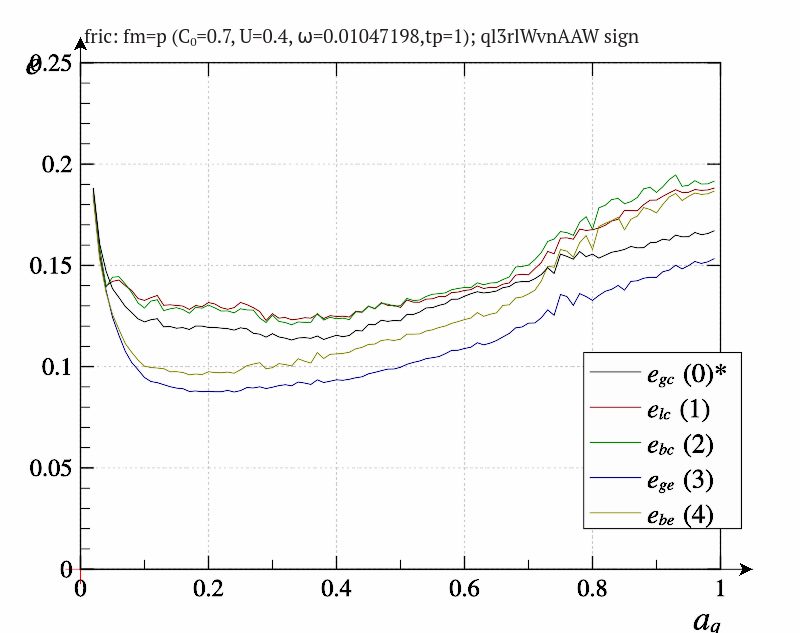
\includegraphics[width=0.49\textwidth]{p/cha/fric/ql3rlWvnAAW/fric_id-p_a_q_sign.png}
    \hfill
    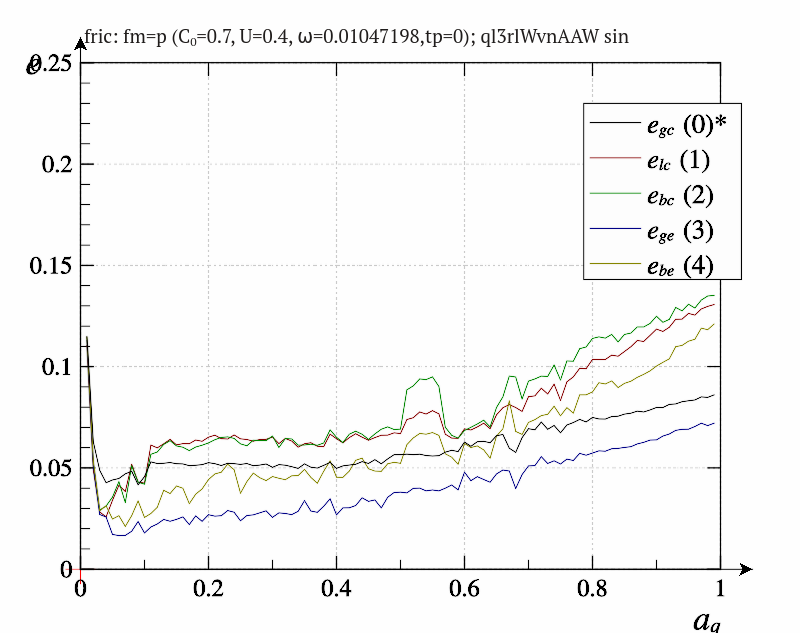
\includegraphics[width=0.49\textwidth]{p/cha/fric/ql3rlWvnAAW/fric_id-p_a_q_sin.png}
  }
  \caption{Зависимости $\overline{e}(a_q)$ при идентификации системы (\ref{atu:eq:dryfric_sys}) группой методов ql3rlWvnAAW.$q_\mathrm{dx}$
   при~(\ref{atu:eq:fric_po_t_sign}) и (\ref{atu:eq:fric_po_t_sin})}
  \label{atu:f:fric_a_q_ql3rlWvnAAW_q_dx}
\end{figure}


Зависимость ошибок идентификации от величины коэффициента масштаба
$q_\gamma$
(рис.~\ref{atu:f:fric_q_gamma_ql3rlWvnAAW_q_dx})
достаточно сильно отличатся от аналогичных для других систем.

\begin{figure}[htb!]
  \centerline{
    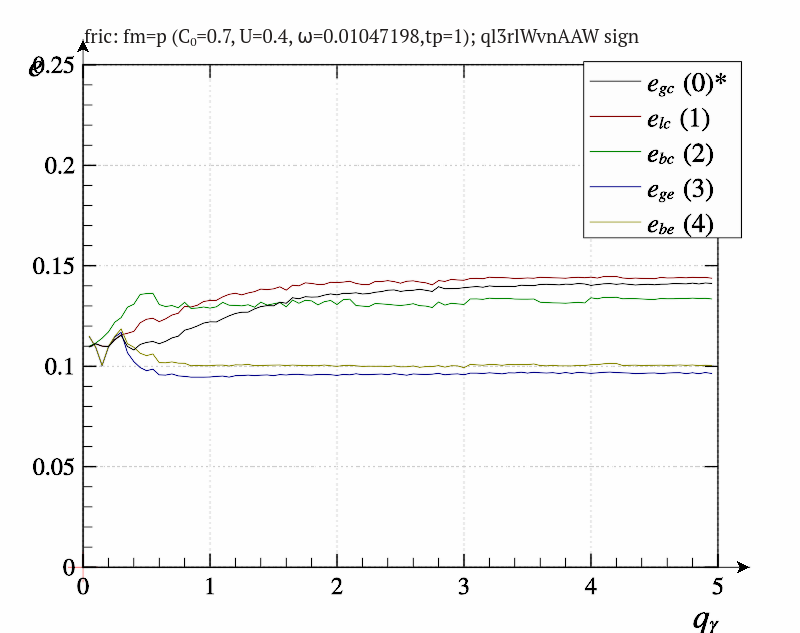
\includegraphics[width=0.49\textwidth]{p/cha/fric/ql3rlWvnAAW/fric_id-p_q_gamma_sign.png}
    \hfill
    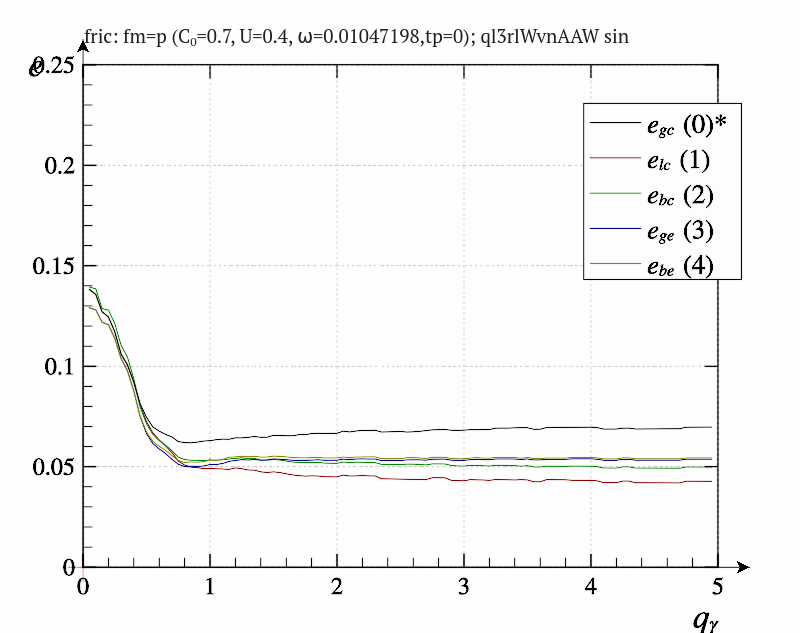
\includegraphics[width=0.49\textwidth]{p/cha/fric/ql3rlWvnAAW/fric_id-p_q_gamma_sin.png}
  }
  \caption{Зависимости $\overline{e}(q_\gamma)$ при идентификации системы (\ref{atu:eq:dryfric_sys}) группой методов ql3rlWvnAAW.$q_\mathrm{dx}$
   при~(\ref{atu:eq:fric_po_t_sign}) и (\ref{atu:eq:fric_po_t_sin})}
  \label{atu:f:fric_q_gamma_ql3rlWvnAAW_q_dx}
\end{figure}

При скачкообразно изменяющемся параметре
нет характерного роста ошибки при избыточной чувствительности
(в ограниченных пределах). При этом существует явное разделение между
результатами работы методов координатора поиска.
Методы, использующие значения $p_e$ от поисковых
агентов, показывают существенно лучшие результаты.
Такое отличие достаточно очевидно, но именно для этой системы
и этих условий
различие столь существенно.
В случае плавно изменяющемся параметра различие не столь существенно,
но при недостаточной чувствительности наилучшие результаты демонстрирует метод $p_{lc}$,
что довольно неожиданно.


На рис.~\ref{atu:f:fric_v_f_ql3rlWvnAAW_q_dx} представлены зависимости ошибки идентификации
от коэффициента скорости поиска $v_f$.
Вид этих зависимостей не проявляет никаких особенностей.
Для плавно меняющегося параметра выигрыш от смещения агентов достигает 800\%,
для скачкообразных изменений --- порядка 20--25\%.

\begin{figure}[htb!]
  \centerline{
    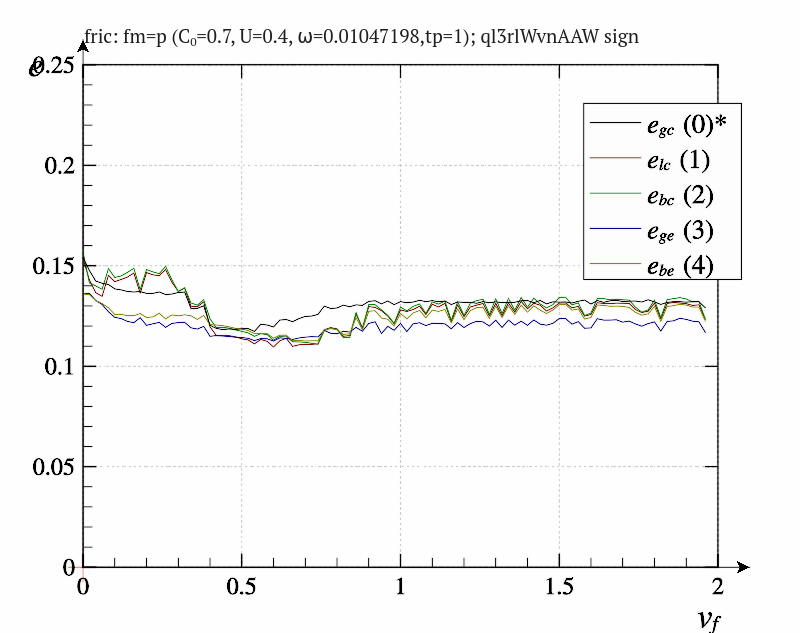
\includegraphics[width=0.49\textwidth]{p/cha/fric/ql3rlWvnAAW/fric_id-p_v_f_sign.png}
    \hfill
    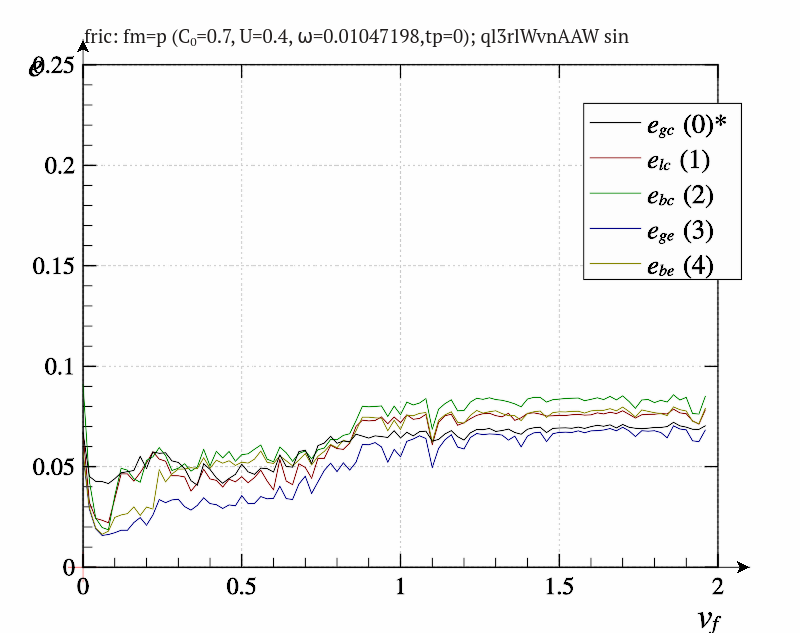
\includegraphics[width=0.49\textwidth]{p/cha/fric/ql3rlWvnAAW/fric_id-p_v_f_sin.png}
  }
  \caption{Зависимости $\overline{e}(v_f)$ при идентификации системы (\ref{atu:eq:dryfric_sys}) группой методов ql3rlWvnAAW.$q_\mathrm{dx}$
   при~(\ref{atu:eq:fric_po_t_sign}) и (\ref{atu:eq:fric_po_t_sin})}
  \label{atu:f:fric_v_f_ql3rlWvnAAW_q_dx}
\end{figure}

Зависимости ошибок идентификации от коэффициента $k_e$,
определяющего равновесное положение агентов
(рис.~\ref{atu:f:fric_k_e_ql3rlWvnAAW_q_dx}),
для данной системы наиболее ярко выражены
при плавном изменении параметра,
что подчёркивает пользу от динамики агентов.
Для скачкообразного изменения параметров динамика
агентов уступает динамике параметра,
и зависимости выражены слабее.

\begin{figure}[htb!]
  \centerline{
    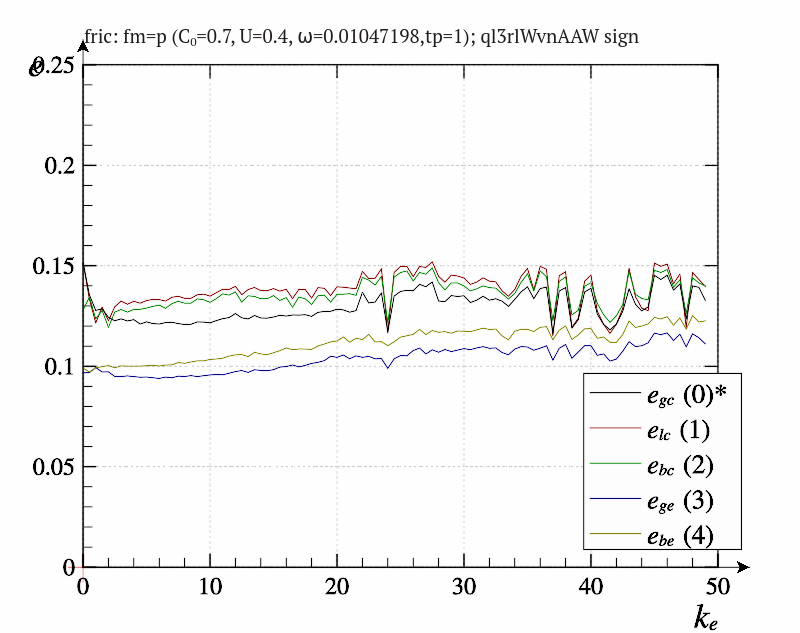
\includegraphics[width=0.49\textwidth]{p/cha/fric/ql3rlWvnAAW/fric_id-p_k_e_sign.png}
    \hfill
    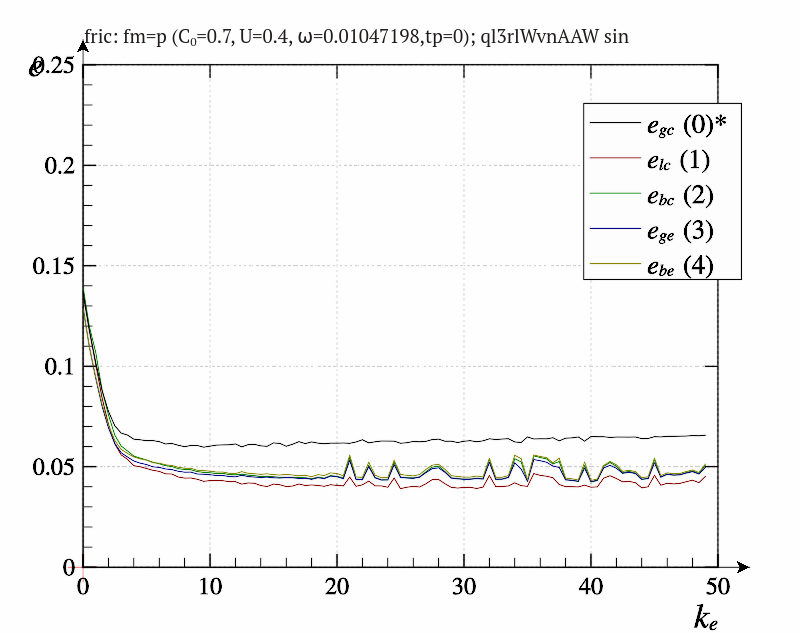
\includegraphics[width=0.49\textwidth]{p/cha/fric/ql3rlWvnAAW/fric_id-p_k_e_sin.png}
  }
  \caption{Зависимости $\overline{e}(k_e)$ при идентификации системы (\ref{atu:eq:dryfric_sys}) группой методов ql3rlWvnAAW.$q_\mathrm{dx}$
   при~(\ref{atu:eq:fric_po_t_sign}) и (\ref{atu:eq:fric_po_t_sin})}
  \label{atu:f:fric_k_e_ql3rlWvnAAW_q_dx}
\end{figure}

Зависимости ошибок от параметра $k_{nl}$
(рис.~\ref{atu:f:fric_k_nl_ql3rlWvnAAW_q_dx}),
определяющего взаимодействие между агентами,
при скачкообразных изменениях параметра
не проявляет существенной зависимости.
Напротив, для плавно изменяющегося значения параметра
существует явно выраженный минимум, соответствующий
балансу между практически свободной динамикой агентов (с учётом ограничений),
и практически фиксированной сеткой агентов.

\begin{figure}[htb!]
  \centerline{
    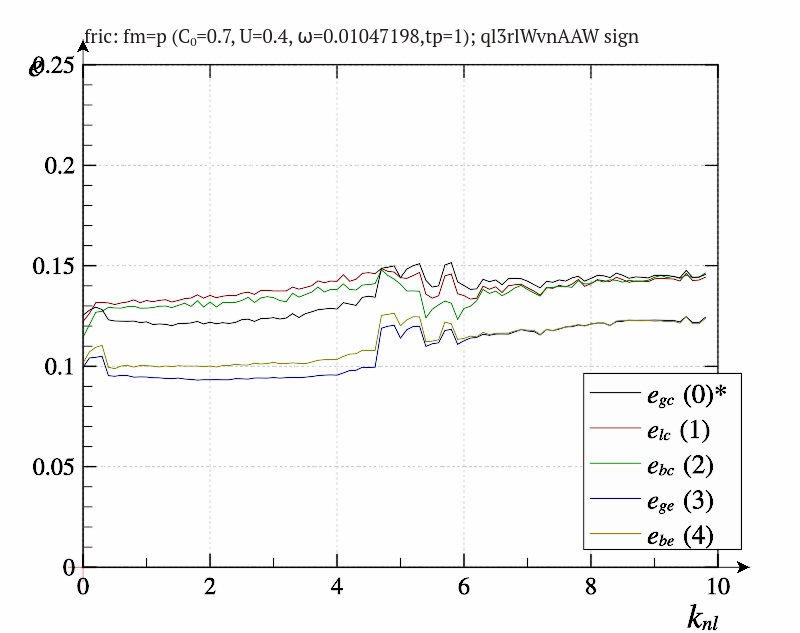
\includegraphics[width=0.49\textwidth]{p/cha/fric/ql3rlWvnAAW/fric_id-p_k_nl_sign.png}
    \hfill
    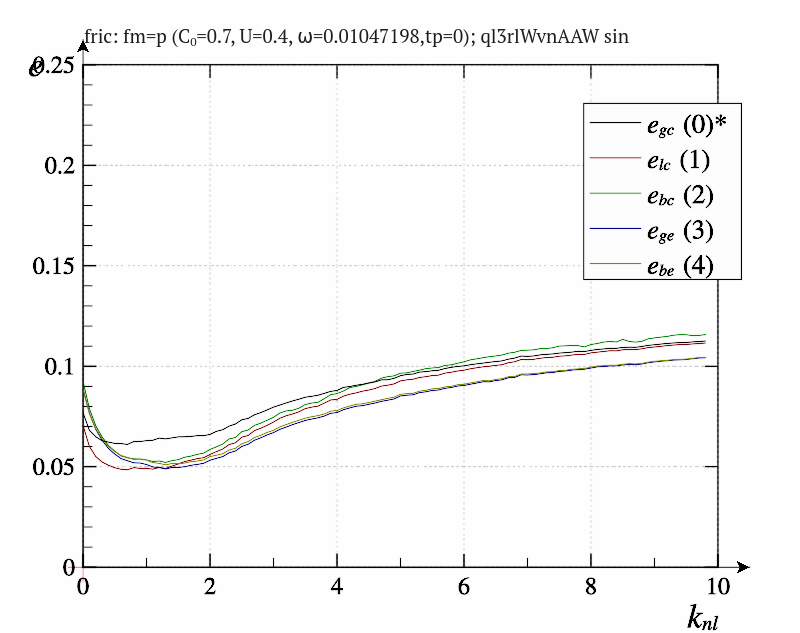
\includegraphics[width=0.49\textwidth]{p/cha/fric/ql3rlWvnAAW/fric_id-p_k_nl_sin.png}
  }
  \caption{Зависимости $\overline{e}(k_{nl})$ при идентификации системы (\ref{atu:eq:dryfric_sys}) группой методов ql3rlWvnAAW.$q_\mathrm{dx}$
   при~(\ref{atu:eq:fric_po_t_sign}) и (\ref{atu:eq:fric_po_t_sin})}
  \label{atu:f:fric_k_nl_ql3rlWvnAAW_q_dx}
\end{figure}


% }}}2

\subsection{Выводы}  % {{{2

В целом, результаты моделирования как динамики системы с силой сухого трения,
и процессов идентификации параметра $f_{dm}$ этой системы,
позволяют сделать следующие выводы:

\begin{itemize}

  \item
    Несмотря на то, что система не проявляет в рассматриваемых условиях хаотическую динамику,
    для идентификации требуется использование специального критерия. Это связано с тем,
    что рассматриваемая система имеет общее свойство с системами динамического хаоса ---
    малые изменения параметра или же входного сигнала могут приводить к
    существенным различиям в динамике.

  \item
    Для данной системы энергетические критерии, аналогичные применённым в предыдущих случаях,
    оказались неприменимы. Критерий, хоть и основанный на измерении производной (после фильтрации),
    оказался работоспособным. В первую очередь это связано с тем, что в основе были положены
    физические принципы, которые для системы с сухим трением, вполне очевидны.

  \item
    Зависимости ошибки идентификации от параметров системы идентификации
    для данной системы выражены достаточно ярко,
    что связано с отсутствием настоящей хаотической динамики.

\end{itemize}



% }}}2



% }}}1

% vim: fdm=marker foldlevel=1 foldignore="%#" fdc=4 ft=tex
